\section{Lecture 10. Exploring Pattern Mining Applications}

Frequent Pattern Mining for Text Data \-— Phrase Mining and Topic Modeling:
\begin{itemize}
\item Strategy 1: Simultaneously Inferring Phrases and Topics
    \begin{itemize}
    \item Generate bag-of-words $\to$ generate sequence of tokens
    \item Bigram topical model [Wallach’06], topical n-gram model [Wang, et al.’07], phrase discovering topic model [Lindsey, et al.’12]
    \end{itemize}
\item Strategy 2: Post Topic Modeling Phrase Construction
    \begin{itemize}
    \item Post bag-of-words model inference, visualize topics with n-grams
    \item Label topic [Mei et al.’07], TurboTopic [Blei \& Lafferty’09], KERT [Danilevsky, et al.’14]
    \end{itemize}
\item Strategy 3: First Phrase Mining then Topic Modeling
    \begin{itemize}
    \item Prior bag-of-words model inference, mine phrases and impose on the bag-of-words model
    \item ToPMine [El-kishky, et al.’15]
    \end{itemize}
\end{itemize}

%--
\subsection{Strategy 1: Simultaneously Inferring Phrases and Topics}
\begin{itemize}
\item \textbf{Bigram Topic Model} [Wallach’06]
    \begin{itemize}
    \item Probabilistic generative model that conditions on previous word and topic when drawing next word
    \end{itemize}

\item Topical N-Grams (\textbf{TNG}) [Wang, et al.’07]
    \begin{itemize}
    \item Probabilistic model that generates words in textual order
    \item Create n-grams by concatenating successive bigrams (a generalization of Bigram Topic Model)
    \end{itemize}

\item Phrase-Discovering LDA\footnote{LDA - Latent Dirichlet Allocation} (\textbf{PDLDA}) [Lindsey, et al.’12]
    \begin{itemize}
    \item Viewing each sentence as a time-series of words, PDLDA posits that the generative parameter (topic) changes periodically
    \item Each word is drawn based on previous m words (context) and current phrase topic
    \end{itemize}
\end{itemize}  

%--
\subsection{Strategy 2: Post Topic Modeling Phrase Construction} 

\subsubsection{TurboTopics}

\textbf{TurboTopics} [Blei \& Lafferty’09] – Phrase construction as a post-processing step to Latent Dirichlet Allocation
\begin{itemize}
\item Perform Latent Dirichlet Allocation on corpus to assign each token a topic label
\item Merge adjacent unigrams with the same topic label by a distribution-free
permutation test on arbitrary-length back-off model
\item End recursive merging when all significant adjacent unigrams have been merged
\end{itemize}

\subsubsection{KERT}
\textbf{KERT} [Danilevsky et al.’14] – Phrase construction as a post-processing step to Latent Dirichlet Allocation
\begin{itemize}
\item Perform frequent pattern mining on each topic
\item Perform phrase ranking based on four different criteria
\end{itemize}

Framework of KERT:
\begin{itemize}
\item Run bag-of-words model inference and assign topic label to each token \item Extract candidate keyphrases within each topic (frequent pattern mining)
\item Rank the keyphrases in each topic
\begin{itemize}
\item Popularity: <<information retrieval>> vs. <<cross-language information retrieval>> 
\item Discriminativeness: only frequent in documents about topic t
\item Concordance: <<active learning>> vs. <<learning classification>>
\item Completeness: <<vector machine>> vs. <<support vector machine>>
\end{itemize}
\end{itemize}

%--
\subsection{Strategy 3: First Phrase Mining then Topic Modeling}

The \textbf{ToPMine} (Topical Phrase Mining) Framework [El-Kishky et al. VLDB’15]:
\begin{itemize}
\item Perform frequent contiguous pattern mining to extract candidate phrases and
their counts
\item Perform agglomerative merging of adjacent unigrams as guided by a significance
score—This segments each document into a “bag-of-phrases”
\item The newly formed bag-of-phrases are passed as input to PhraseLDA, an extension of LDA, that constrains all words in a phrase to each sharing the same latent topic
\end{itemize}

\subsubsection{Phrase Mining: Frequent Pattern Mining + Statistical Analysis}

Significance score:
\begin{equation*}
\alpha(P_1, P_2) \approx \frac{f(P_1 \bullet P_2) - \mu_0(P_1, P_2)}{\sqrt{f(P_1 \bullet P_2)}}
\end{equation*}

\begin{figure}[H]
    \centering
    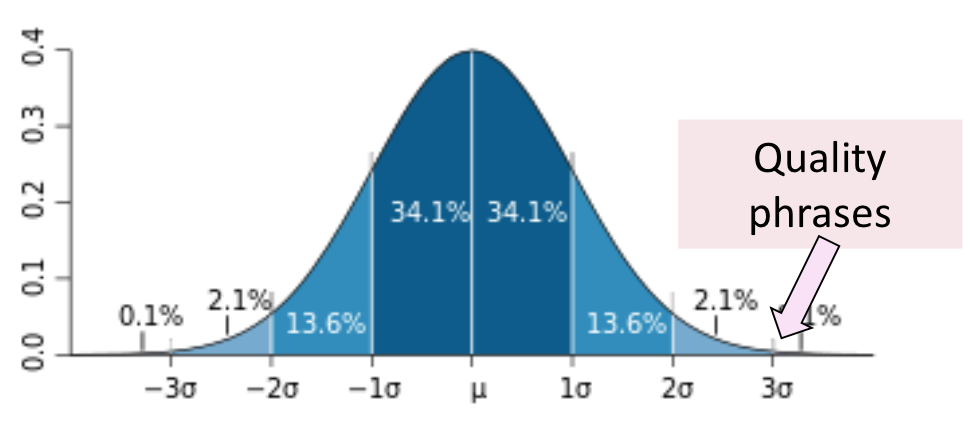
\includegraphics[width=0.55\linewidth]{topmine_significance.png}
    \caption{Significance score}
\end{figure}

\begin{figure}[H]
    \centering
    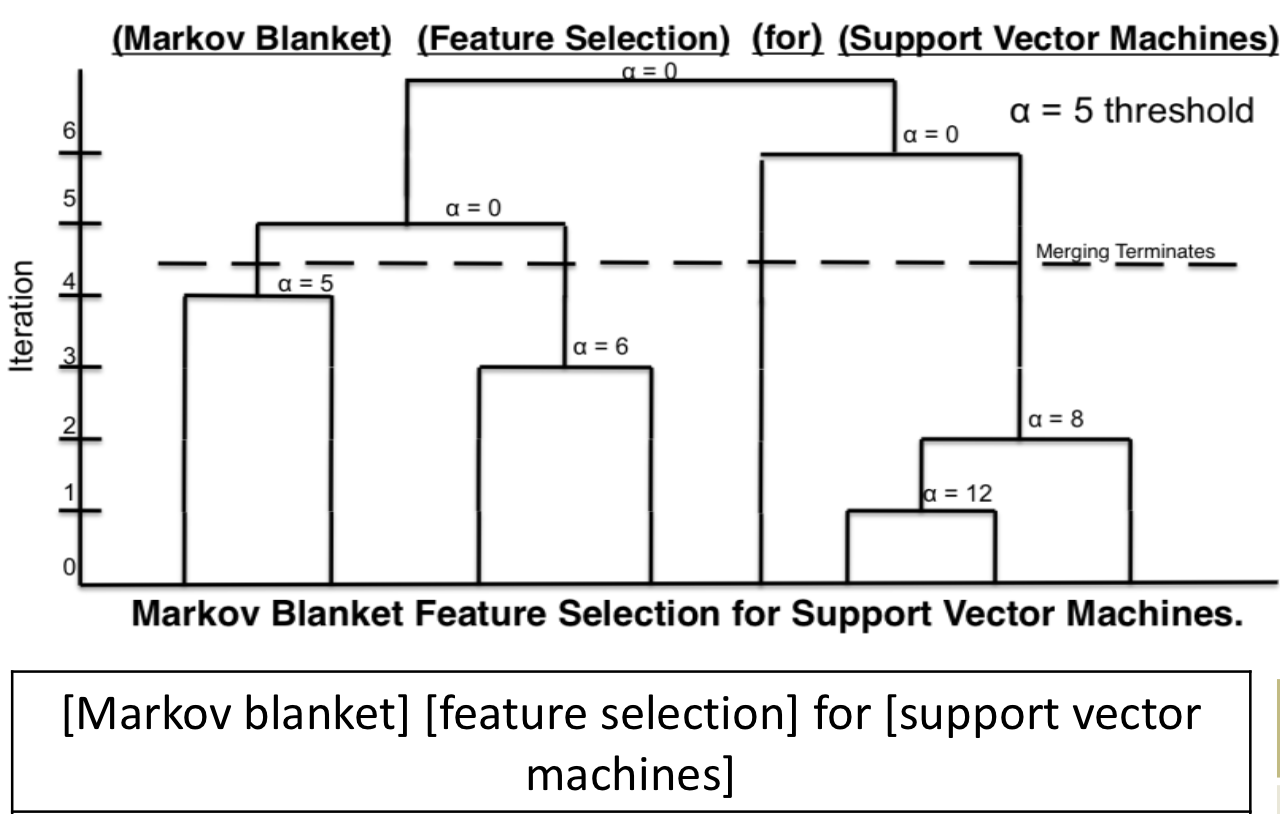
\includegraphics[width=0.6\linewidth]{topmine_phrases.png}
    \caption{Phrase Mining}
\end{figure}

%--
\subsection{Recommended Readings}
\begin{itemize}
\item M. Danilevsky, C. Wang, N. Desai, X. Ren, J. Guo, J. Han. <<Automatic Construction and Ranking of Topical Keyphrases on Collections of Short Documents>>, SDM’14
\item X. Wang, A. McCallum, X. Wei. Topical n-grams: Phrase and topic discovery, with an application to information retrieval, ICDM’07
\item R. V. Lindsey, W. P. Headden, III, M. J. Stipicevic. A phrase-discovering topic model using hierarchical pitman-yor processes, EMNLP-CoNLL’12.
\item Q. Mei, X. Shen, C. Zhai. Automatic labeling of multinomial topic models, KDD’07
\item D. M. Blei and J. D. Lafferty. Visualizing Topics with Multi-Word Expressions, arXiv:0907.1013, 2009
\item M. Danilevsky, C. Wang, N. Desai, J. Guo, J. Han. Automatic Construction and Ranking of Topical Keyphrases on Collections of Short Documents, SDM’14
\item A. El-Kishky, Y. Song, C. Wang, C. R. Voss, J. Han. Scalable Topical Phrase Mining from Text Corpora, VLDB'15
\item K. Church, W. Gale, P. Hanks, D. Hindle. Using Statistics in Lexical Analysis. In U. Zernik (ed.), Lexical Acquisition: Exploiting On-Line Resources to Build a Lexicon. Lawrence Erlbaum, 1991
\end{itemize}

